\documentclass[12pt, a4paper]{article}

\usepackage[utf8]{inputenc}
\usepackage[T1]{fontenc}
\usepackage[english]{babel}
\usepackage{amsmath}
\usepackage{amssymb}
\usepackage{graphicx}
\usepackage{booktabs}
\usepackage{multirow}
\usepackage{hyperref}
\usepackage{geometry}
\usepackage{caption}
\usepackage{subcaption}
\usepackage{xcolor}
\usepackage{tabularx}
\usepackage{titlesec}
\usepackage{listings}
\usepackage{float}
\usepackage{tikz}
\usepackage{tikzpeople}
\usepackage{caption}
\usetikzlibrary{arrows.meta, shapes.geometric, shapes.misc, fit, positioning, backgrounds, calc}

\geometry{margin=2.5cm}

\hypersetup{
    colorlinks=true,
    linkcolor=black,
    citecolor=black,
    urlcolor=blue,
    pdftitle={Report SAR},
    pdfauthor={Donato Festa}
}

% Title Format
\titleformat{\section}
  {\normalfont\Large\bfseries}{\thesection}{1em}{}
\titleformat{\subsection}
  {\normalfont\large\bfseries}{\thesubsection}{1em}{}

\begin{document}

% =========================================================
% FRONTESPIZIO
% =========================================================
\begin{titlepage}
    \begin{center}
        
\includegraphics[scale=0.48]{uniba_logo.png}\\
        \vspace{1cm}
        {\Large \textbf{Computer Science Department}}\\
        \vspace{0.5cm}
        {\Large \textbf{Master's Degree in Computer Science}}\\
        \hrulefill \\
        \vspace{2cm}
        {\Large Computer Vision}\\
        \vspace{25pt}
        {\huge \textbf{Overcoming Spatial Misalignment in Aerial RGB-IR Object Detection}}
        \\ 
        \vspace{0.5cm}
   
        \vfill
        \centering
        \begin{tabularx}{\textwidth}{@{}Xr@{}}
          {\large Student:} &
          {\large Donato Festa} \\[0.5cm] 
          {\large Professor:} &
          {\large Giovanna Castellano} \\ 
        \end{tabularx}
        \textcolor{white}{.} \\ 
        \hrulefill \\
        \vspace{0.2cm}
        {\large \textbf{Academic Year 2025-2026}}
    \end{center}
  \end{titlepage}

\tableofcontents
\newpage

%-------------------------------------------------------
\begin{abstract}
This report investigates multimodal RGB-IR object detection for Search and Rescue (SAR) operations conducted via Unmanned Aerial Vehicles (UAVs), addressing the geometric misalignment between visible and thermal sensors that limits naive fusion strategies. Starting from an RT-DETR baseline with Additive Feature Fusion and Modal Dropout (0.357 mAP@50 in fusion mode, with balanced single-modality robustness), this work pursues three complementary architectural directions.

First, a \textit{Feature Alignment Module (FAM)} based on Deformable Convolutions is introduced on top of RT-DETR: RGB features guide the spatial realignment of thermal features before additive fusion, raising single-modality robustness to a new best of 0.263 mAP@50 on IR-only data while achieving 0.396 mAP@50 in fusion mode. Second, a \textit{Hybrid CMX} architecture (base CMX augmented with this same Feature Alignment Module and a 2D Positional Encoding) is designed to address three structural deficiencies identified in the pure CMX framework: sensor misalignment, attention ghosting, and a P3 computational bottleneck. The hybrid design substantially recovers from the collapse of pure CMX (0.032 mAP@50) to 0.145 mAP@50, confirming the diagnosis while remaining below the baseline. Third, \textit{Deformable DETR} is adapted for RGB-IR fusion through Channel Concatenation with a non-linear fusion block (Conv$1\times1$ + GroupNorm + ReLU), and the same FAM alignment strategy is transferred to this architecture; due to observed run-to-run non-determinism in the deformable attention mechanism, results are reported as median and range over five random seeds, with FAM improving the median fusion score from 0.249 to 0.294 mAP@50.

Across all experiments, a unifying conclusion emerges: on small, geometrically misaligned RGB-IR datasets such as WiSARD, lightweight heuristic alignment operations consistently outperform heavy attention-based fusion frameworks, and explicit geometric correction (FAM) provides a more reliable and interpretable improvement path than increasing fusion complexity.
\end{abstract}
 
\newpage
 
%-------------------------------------------------------
\section{Introduction}
\label{sec:intro}
 
Search and Rescue (SAR) operations in wilderness environments impose severe constraints on vision systems: targets are typically small relative to the field of view, illumination varies drastically between day and night, and on-board computational resources are limited. Equipping UAVs with both a visible-spectrum (RGB) camera and a thermal infrared (IR) sensor is a well-established strategy to mitigate these issues, since each modality captures complementary informations (texture and colour from RGB, heat signatures from IR).
 
However, the joint use of two sensors introduces a set of domain-specific challenges that are not present in standard single-modality detection:
 
\begin{itemize}
    \item \textbf{Sensor misalignment.} RGB and IR cameras are physically separate devices mounted on the same UAV. At typical UAV flight altitudes, the parallax between the two lenses produces non-negligible geometric offsets between the two image streams. This misalignment is not constant: it varies with altitude, gimbal angle, and the depth of the scene, making it impossible to correct with a fixed homography.
    \item \textbf{Thermal crossover.} During certain times of day, the surface temperature of terrain and vegetation equalises with that of human subjects, causing the thermal contrast of targets to vanish entirely. In these conditions, the IR sensor becomes uninformative and the system must fall back to RGB alone.
    \item \textbf{Sensor failure and modal collapse.} In real-world deployments, either sensor may be unavailable - due to hardware failure, obstructions (smoke, fog), or environmental conditions (total darkness for RGB). A multimodal model trained exclusively on paired data develops a strong co-adaptation between the two input streams, failing catastrophically when one is absent. This phenomenon is referred to as \textit{modal collapse}.
    \item \textbf{Small target size.} Human subjects occupy a minimal fraction of the image area at operational UAV altitudes, making detection inherently difficult and sensitive to any source of noise or misalignment in the input features.
\end{itemize}
 
\subsection{Prior Work and Motivation}
 
A prior investigation on this project addressed the challenges of thermal crossover and sensor failure using the WiSARD (Wilderness Search and Rescue Dataset) dataset, training a standard DETR~\cite{carion2020detr} model under a Modal Dropout regime. That work established that \textit{Modal Dropout}~\cite{neverova2015moddrop} - which stochastically replaces one or both input modalities with zero tensors during training - is critical to prevent modal collapse: without it, a model trained exclusively on paired RGB-IR data achieves 0 mAP@50 when tested on a single modality at inference time. The optimal dropout setting was found to be $P(\text{IR}) = 20\%$, $P(\text{RGB}) = 20\%$, $P(\text{Fusion}) = 60\%$, yielding the best trade-off between fusion accuracy and single-modality robustness across multiple training-set compositions.

Building on this finding, the investigation turned to RT-DETR~\cite{xu2023rtdetr}, a real-time detection transformer, adapted for RGB-IR fusion through an Additive Feature Fusion scheme. Section~\ref{sec:rtdetr_baseline} presents this baseline in detail, together with the subsequent attempt to replace additive fusion with the CMX framework~\cite{zhang2023cmx}, which collapsed to 0.032 mAP@50 due to destructive cross-modal interference caused by sensor misalignment.
This report pursues the following core objectives:
\begin{enumerate}
    \item \textbf{Enhancing RT-DETR via Explicit Alignment:} Integrate an explicit Feature Alignment Module (FAM) based on Deformable Convolutions~\cite{zhu2019dcnv2} between the dual backbone and the additive fusion step to resolve spatial misalignment and maximize multimodal fusion accuracy.
    \item \textbf{Remedying CMX Structural Deficiencies:} Design and evaluate a hybrid pipeline, built on top of the same FAM, to mitigate the three structural failure modes of the pure CMX framework, namely sensor misalignment, spatial ghosting, and the P3 computational bottleneck.
    \item \textbf{Evaluating Deformable Attention Baselines:} Assess Deformable DETR~\cite{zhu2020deformable} as an alternative sparse multi-scale fusion backbone, and analyze the transferability and stability of the FAM alignment strategy within its architecture.
\end{enumerate}
 
\subsection{Dataset and Nomenclature}
\label{subsec:nomenclature}
 
In this work all experiments use the WiSARD dataset. To evaluate model performance under different sensor availability scenarios, the dataset is physically organised into distinct subfolders. The following nomenclature is used consistently throughout this report:
 
\begin{itemize}
    \item $D_{\text{RGBa-IRs}}$ \textbf{(Full RGB + Sync IR):} Combines all available RGB images (including unpaired ones) with the synchronised thermal subset. Designed to maximise the use of visual information.
    \item $D_{\text{RGBs-IRa}}$ \textbf{(Full IR + Sync RGB):} Combines all available IR images (including unpaired ones) with the synchronised RGB subset. Used to evaluate the impact of a training set biased towards the thermal modality.
    \item $D_{\text{RGB-IR}}$ \textbf{(Strictly Paired):} Contains only perfectly synchronised RGB-IR image pairs. Used to isolate the effectiveness of pure fusion without the bias introduced by unpaired data.
    \item $D$ \textbf{(Whole Dataset):} The complete union of all available data: RGB-only images, IR-only images, and synchronised pairs. Represents the most diverse and challenging generalisation scenario.
    \item $D_{\text{IRo}}$ \textbf{(IR-only):} Test subset in which visible-spectrum information has been removed or zeroed out, simulating a night scenario or RGB camera failure. The model receives only the thermal channel.
    \item $D_{\text{VISo}}$ \textbf{(Visible-only):} Test subset in which thermal information is absent (e.g., thermal crossover or IR sensor failure). The model operates exclusively on the visible spectrum.
\end{itemize}
 
This distinction is crucial for the analysis: comparing results across these subsets allows us to determine whether the model has genuinely learned independent unimodal representations or has collapsed into a joint-modality dependency.

%-------------------------------------------------------
\section{RT-DETR with Additive Feature Fusion}

Following the DETR experiments, the investigation moved to RT-DETR~\cite{xu2023rtdetr} (Real-Time DEtection TRansformer), motivated by the need to retain the robustness benefits of Modal Dropout while achieving real-time inference speed. RT-DETR replaces dense self-attention with an efficient hybrid encoder that decouples intra-scale interaction (AIFI, applied only to the lowest-resolution feature level) from cross-scale fusion (CCFM), drastically reducing inference latency.

\label{sec:rtdetr_baseline}

\begin{figure}[H]
    \centering
    \includegraphics[width=0.9\textwidth]{rtdetr_schema.png}
    \caption{RT-DETR architecture~\cite{xu2023rtdetr} with Additive Feature Fusion. In our approach two independent ResNet-50vd backbones process the RGB and IR streams separately. The resulting multi-scale feature maps (P3, P4, P5) are fused element-wise before entering the Efficient Hybrid Encoder, which decouples intra-scale interaction (AIFI) from cross-scale fusion (CCFM).}
    \label{fig:rtdetr_baseline_schema}
\end{figure}

\subsection{Architecture}

To adapt RT-DETR to the multimodal setting, an \textit{Additive Feature Fusion} scheme was adopted:
\begin{enumerate}
    \item \textbf{Dual Backbone.} Two independent ResNet-50vd backbones extract multi-scale feature maps ($P3$, $P4$, $P5$) separately from the RGB and IR streams.
    \item \textbf{Fusion.} Corresponding feature maps are fused via element-wise summation:
    \begin{equation}
        F^{(i)}_{\text{fused}} = F^{(i)}_{\text{RGB}} + F^{(i)}_{\text{IR}}, \qquad i \in \{P3, P4, P5\}
    \end{equation}
    \item \textbf{Hybrid Encoder.} The fused features are passed to the standard RT-DETR hybrid encoder.
\end{enumerate}

This fusion strategy was preferred over concatenation-based alternatives because it preserves the native spatial alignment and geometry required by the hybrid encoder, introduces no additional parameters, and avoids the training instability that a heavier fusion module could cause when fine-tuning an ImageNet/COCO-pretrained backbone on a dataset as small as WiSARD. The model was trained with the optimal Modal Dropout schedule identified in prior work ($P(\text{IR})=20\%$, $P(\text{RGB})=20\%$, $P(\text{Fusion})=60\%$).

\subsection{Results}

\begin{table}[h]
\centering
\caption{RT-DETR (Additive Fusion) trained for 10 epochs on full-resolution images, across confidence thresholds.}
\label{tab:rtdetr_base_10}
\begin{tabular}{lccc}
\toprule
\textbf{Test Set} & \textbf{Threshold} & \textbf{mAP@50 (RT-DETR)} & \textbf{mAP@50 (DETR)} \\
\midrule
$D_{\text{RGB-IR}}$ & 0.01 & \textbf{0.357} & \multirow{3}{*}{0.417} \\
$D_{\text{RGB-IR}}$ & 0.05 & 0.357 & \\
$D_{\text{RGB-IR}}$ & 0.10 & 0.356 & \\
\midrule
$D_{\text{IRo}}$  & 0.01 & 0.252 & 0.173 \\
$D_{\text{VISo}}$ & 0.01 & 0.246 & -- \\
\bottomrule
\end{tabular}
\end{table}

\begin{table}[h]
\centering
\caption{RT-DETR (Additive Fusion) trained for 25 epochs on full-resolution images, across confidence thresholds.}
\label{tab:rtdetr_base_25}
\begin{tabular}{lccc}
\toprule
\textbf{Test Set} & \textbf{Threshold} & \textbf{mAP@50 (RT-DETR)} & \textbf{mAP@50 (DETR)} \\
\midrule
$D_{\text{RGB-IR}}$ & 0.01 & 0.321 & \multirow{3}{*}{0.417} \\
$D_{\text{RGB-IR}}$ & 0.05 & 0.287 & \\
$D_{\text{RGB-IR}}$ & 0.10 & 0.246 & \\
\midrule
$D_{\text{IRo}}$  & 0.01 & 0.262 & 0.173 \\
$D_{\text{VISo}}$ & 0.01 & 0.264 & -- \\
\bottomrule
\end{tabular}
\end{table}

The 10-epoch model outperforms the 25-epoch model on the fusion test set (0.357 vs.\ 0.321), suggesting mild overfitting beyond epoch 10 - consistent with the limited size of WiSARD - while the 25-epoch model shows a slight edge on the single-modality subsets. At 10 epochs, performance is nearly identical across thresholds 0.01 to 0.10 (0.357 $\to$ 0.356), indicating high-confidence predictions; at 25 epochs, sensitivity to the threshold increases markedly (0.321 $\to$ 0.246), a symptom of less stable predictions.

Compared to the DETR baseline, RT-DETR trades a moderate drop in fusion accuracy (0.357 vs.\ 0.417, $-14\%$) for a substantial gain in single-modality robustness (IR-only: 0.252 vs.\ 0.173, $+46\%$), confirming that the combination of Additive Fusion and Modal Dropout transfers effectively to the real-time architecture. The 10-epoch configuration is adopted as the reference baseline for the remainder of this report.

\newpage

%-------------------------------------------------------
\section{Feature Alignment Module (FAM) on RT-DETR}
\label{sec:fam}

\subsection{Motivation}
\label{subsec:fam_motivation}

Despite its efficiency, the RT-DETR baseline presented in Section~\ref{sec:rtdetr_baseline} is limited by the fact that RGB and IR feature maps are summed element-by-element without any correction for the inherent spatial misalignment between the two sensors. Given the experimental evidence that misalignment is a dominant performance bottleneck (confirmed, in prior work, by the failure of a tiling-based scale-increase strategy to recover accuracy), an explicit alignment module was designed and inserted between the dual backbone outputs and the additive fusion step of the same RT-DETR architecture shown in Figure~\ref{fig:rtdetr_baseline_schema}.

\subsection{Architecture}

\begin{figure}[htbp]
\centering
\resizebox{0.85\textwidth}{!}{%
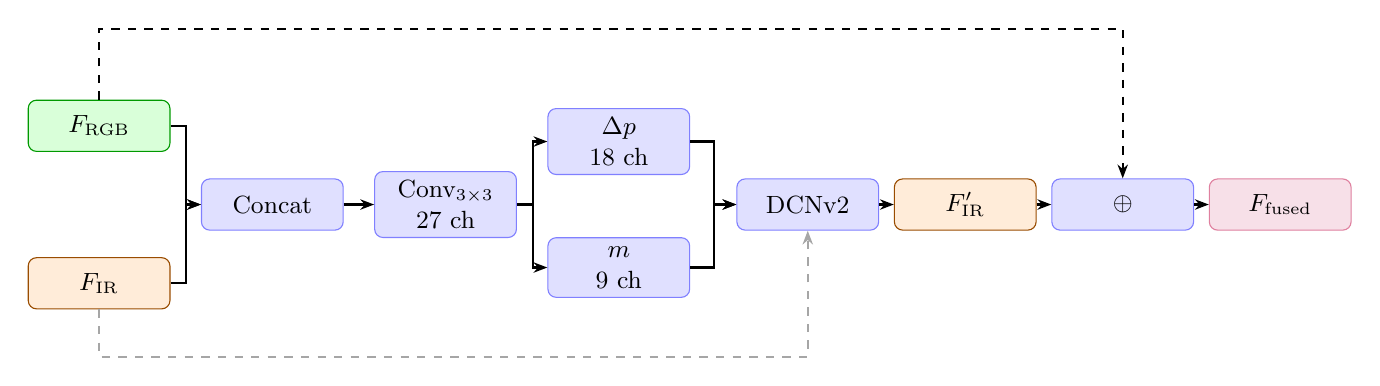
\begin{tikzpicture}[
    box/.style={draw, rounded corners=3pt, minimum width=1.8cm, minimum height=0.65cm, align=center, font=\small},
    rgbbox/.style={box, fill=green!15,  draw=green!60!black},
    irbox/.style= {box, fill=orange!15, draw=orange!60!black},
    opbox/.style= {box, fill=blue!12,   draw=blue!50},
    outbox/.style={box, fill=purple!12, draw=purple!50},
    arrow/.style={-{Stealth[length=5pt]}, thick}
]
\node[rgbbox] (rgb)     at (0,    1.0) {$F_{\text{RGB}}$};
\node[irbox]  (ir)      at (0,   -1.0) {$F_{\text{IR}}$};
\node[opbox]  (concat)  at (2.2,  0.0) {Concat};
\node[opbox]  (oconv)   at (4.4,  0.0) {Conv$_{3\times3}$\\27 ch};
\node[opbox]  (delta)   at (6.6,  0.8) {$\Delta p$\\18 ch};
\node[opbox]  (mask)    at (6.6, -0.8) {$m$\\9 ch};
\node[opbox]  (dcn)     at (9.0,  0.0) {DCNv2};
\node[irbox]  (iralign) at (11.0, 0.0) {$F'_{\text{IR}}$};
\node[opbox]  (add)     at (13.0, 0.0) {$\oplus$};
\node[outbox] (out)     at (15.0, 0.0) {$F_{\text{fused}}$};

% RGB bypass
\draw[arrow, dashed] (rgb.north) -- ++(0, 0.9) -| (add.north);

% IR direct feed to DCNv2 — loops under everything
\draw[arrow, dashed, gray!70] (ir.south) -- ++(0, -0.6) -| (dcn.south);

% Main arrows
\draw[arrow] (rgb.east)   -- ++(0.2,0) |- (concat.west);
\draw[arrow] (ir.east)    -- ++(0.2,0) |- (concat.west);
\draw[arrow] (concat)     -- (oconv);
\draw[arrow] (oconv.east) -- ++(0.2,0) |- (delta.west);
\draw[arrow] (oconv.east) -- ++(0.2,0) |- (mask.west);
\draw[arrow] (delta.east) -- ++(0.3,0) |- (dcn.west);
\draw[arrow] (mask.east)  -- ++(0.3,0) |- (dcn.west);
\draw[arrow] (dcn)        -- (iralign);
\draw[arrow] (iralign)    -- (add);
\draw[arrow] (add)        -- (out);
\end{tikzpicture}%
}
\caption{Feature Alignment Module (FAM). The RGB and IR feature maps are concatenated and fed into a $3\times3$ convolution that predicts spatial offsets $\Delta p$ (18 ch) and modulation scalars $m$ (9 ch). The offsets are applied to $F_{\text{IR}}$ via DCNv2, producing the aligned $F'_{\text{IR}}$, which is then summed with $F_{\text{RGB}}$.}
\label{fig:fam_diagram}
\end{figure}

The Feature Alignment Module (FAM) is inserted between the dual backbone outputs and the additive fusion step. For each feature pyramid level $i$, the module computes spatially-adaptive sampling offsets from the RGB features and uses them to warp the IR features via Deformable Convolution v2 (DCNv2) \cite{zhu2019dcnv2}. The three sub-steps are:

\paragraph{1. Offset Learning.} The RGB and IR feature maps are concatenated along the channel dimension and passed through a standard $3\times3$ convolution that produces 27 output channels:
\begin{equation}
    [\Delta p,\, m] = \text{Conv}_{3\times3}\!\left(\text{Concat}(F_{\text{RGB}},\, F_{\text{IR}})\right)
\end{equation}
The 27 channels encode: 18 spatial offsets $\Delta p$ (two coordinates $\times$ 9 kernel points) and 9 modulation scalars $m$ (one per kernel point).

\paragraph{2. Deformable Alignment.} The learned offsets and modulation scalars are applied to $F_{\text{IR}}$ through a DCNv2 layer:
\begin{equation}
    F'_{\text{IR}}(p) = \sum_{k=1}^{K} w_k \cdot F_{\text{IR}}\!\left(p + p_k + \Delta p_k\right) \cdot m_k
\end{equation}
where $p$ is the current spatial position, $p_k$ is the $k$-th fixed kernel offset, and $\Delta p_k$ is the learned correction. The offset convolution weights are initialised to zero, so the FAM starts as an identity mapping and gradually learns the geometric correction. The module's parameters are registered in the model constructor, so the optimiser updates them consistently from the very first training iteration.

\paragraph{3. Additive Fusion.} The aligned IR feature map is added to the original RGB features:
\begin{equation}
    F^{(i)}_{\text{fused}} = F^{(i)}_{\text{RGB}} + F^{(i)\prime}_{\text{IR}}
\end{equation}

\subsection{Qualitative Analysis}

Figure~\ref{fig:fam_qualitative} shows representative predictions of the model using the FAM on two scenarios. In the Fusion scenario (a), the model jointly leverages RGB texture and thermal signatures to localize persons in a cluttered mountain environment, despite low individual confidence scores. In the IR-only scenario (b), the model successfully detects the subject relying exclusively on the thermal channel, demonstrating that Modal Dropout preserves a functional thermal processing pathway even after FAM is introduced.

\begin{figure}[H]
    \centering

    \begin{minipage}{0.42\textwidth}
        \centering \textbf{\small Ground Truth}
    \end{minipage}
    \hspace{0.02\textwidth}
    \begin{minipage}{0.42\textwidth}
        \centering \textbf{\small Prediction (RT-DETR + FAM)}
    \end{minipage}

    \vspace{0.15cm}

    \begin{subfigure}[t]{0.42\textwidth}
        \centering
        \includegraphics[width=\textwidth]{rtdetr_fam_visir_gt.png}
    \end{subfigure}
    \hspace{0.02\textwidth}
    \begin{subfigure}[t]{0.42\textwidth}
        \centering
        \includegraphics[width=\textwidth]{rtdetr_fam_visir_pred.png}
    \end{subfigure}

    \vspace{0.05cm}
    {\small\textit{(a) Scenario Fusion (Input RGB + IR)}}

    \vspace{0.2cm}

    \begin{subfigure}[t]{0.42\textwidth}
        \centering
        \includegraphics[width=\textwidth]{rtdetr_fam_ir_gt.png}
    \end{subfigure}
    \hspace{0.02\textwidth}
    \begin{subfigure}[t]{0.42\textwidth}
        \centering
        \includegraphics[width=\textwidth]{rtdetr_fam_ir_pred.png}
    \end{subfigure}

    \vspace{0.05cm}
    {\small\textit{(b) Scenario IR-only}}

\end{figure}

\begin{center}
    \captionof{figure}{\textbf{Qualitative analysis of RT-DETR + FAM.} Comparison between ground truth annotations (left) and model predictions (right). Bounding boxes correspond to raw predictions at threshold 0.01; confidence scores are low but spatial localization is consistent with ground truth.}
    \label{fig:fam_qualitative}
\end{center}

\subsection{Results}

\begin{table}[htbp]
\centering
\caption{RT-DETR + FAM vs.\ RT-DETR Baseline and DETR baselines.}
\label{tab:fam_results}
\begin{tabular}{lccc}
\toprule
\textbf{Model} & \textbf{Test Set} & \textbf{Threshold} & \textbf{mAP@50} \\
\midrule
\multirow{4}{*}{RT-DETR + FAM}
    & $D_{\text{RGBa-IRs}}$ & 0.01 & 0.396 \\
    & $D_{\text{RGBa-IRs}}$ & 0.10 & 0.394 \\
    & $D_{\text{IRo}}$      & 0.01 & \textbf{0.263} \\
    & $D_{\text{VISo}}$     & 0.01 & 0.262 \\
\midrule
\multirow{3}{*}{RT-DETR Baseline}
    & $D_{\text{RGBa-IRs}}$ & 0.01 & 0.357 \\
    & $D_{\text{IRo}}$      & 0.01 & 0.252 \\
    & $D_{\text{VISo}}$     & 0.01 & 0.246 \\
\midrule
DETR & $D_{\text{RGBa-IRs}}$ & 0.05 & \textbf{0.417} \\
     & $D_{\text{IRo}}$      & 0.01 & 0.173 \\
\bottomrule
\end{tabular}
\end{table}

FAM improves the fusion score over the RT-DETR Baseline (0.396 vs.\ 0.357, $+11\%$) while simultaneously raising IR-only robustness to a new best of 0.263 mAP@50 (vs.\ 0.252, $+4\%$) and leaving visible-only performance essentially unchanged (0.262 vs.\ 0.246). This indicates that the alignment module improves the geometric quality of thermal features without resorting to excessive use of RGB, which a purely additive scheme would risk if the IR features were spatially distorted.

Compared to the DETR baseline, RT-DETR + FAM falls short in fusion mode (0.396 vs.\ 0.417) but closes a substantial part of the gap relative to the plain RT-DETR baseline, while retaining much stronger single-modality performance (IR-only: 0.263 vs.\ 0.173, $+52\%$). The negligible drop between threshold 0.01 and 0.10 (0.396 vs.\ 0.394) again reflects high prediction confidence.

\newpage 

%-------------------------------------------------------
\section{Hybrid CMX: FAM + CM-FRM + FFM + Positional Encoding}
\label{sec:hybrid_cmx}

\subsection{Motivation: Three Structural Deficiencies of Pure CMX}

The failure of the pure CMX framework (0.032 mAP@50 on fusion, vs.\ 0.357 for RT-DETR Baseline) was not attributed to the concept of cross-modal rectification per se, but to three structural incompatibilities with the WiSARD domain:

\begin{enumerate}
    \item \textbf{Misalignment and Parallax.} The CM-FRM rectification module assumes near-perfect pixel-level registration. When RGB and IR pixels at the same spatial location correspond to physically different scene points, cross-modal calibration mixes the target's thermal signature with background clutter, causing destructive interference. This is a known failure mode in datasets acquired from UAVs at altitude, where the parallax between sensors mounted on the same gimbal is non-negligible.
    \item \textbf{Spatial Context Loss in FFM.} The cross-attention fusion module (FFM) flattens spatial tokens, temporarily stripping them of 2D positional information. Without explicit position encoding, the attention mechanism can match thermal tokens to semantically similar but spatially mislocated RGB regions (e.g., warm patches of ground rather than human subjects), a phenomenon referred to here as \textit{attention ghosting}.
    \item \textbf{P3 Computational Bottleneck.} The $\mathcal{O}(N^2)$ complexity of full self-attention at the highest-resolution feature level P3 (which is critical for detecting small targets) forces a linear convolutional bypass. When the feature maps fed into this bypass are spatially misaligned, the bypass irreversibly destroys the small-target signatures.
\end{enumerate}

\newpage

\subsection{Hybrid Architecture: TripleStep Pipeline}

To address these three deficiencies simultaneously, a \textbf{Hybrid CMX} architecture was designed. The fusion pipeline for each feature level $i \in \{P3, P4, P5\}$ follows three sequential steps:
\begin{equation}
    [F^{(i)}_{\text{RGB}},\, F^{(i)}_{\text{IR}}]
    \;\xrightarrow{\text{FAM}}\;
    [F^{(i)}_{\text{RGB}},\, \tilde{F}^{(i)}_{\text{IR}}]
    \;\xrightarrow{\text{CM-FRM}}\;
    [F^{(i)\prime}_{\text{RGB}},\, F^{(i)\prime}_{\text{IR}}]
    \;\xrightarrow{\text{FFM+PE}}\;
    F^{(i)}_{\text{fused}}
\end{equation}


\begin{figure}[H]

\centering

\includegraphics[width=\textwidth]{cmx_schema.png}

\caption{Architecture of the CMX framework \cite{zhang2023cmx}. (a) Overall pipeline with alternating CM-FRM and FFM modules at each feature level. (b) CM-FRM: channel-wise and spatial-wise cross-modal rectification. (c) FFM: two-stage cross-attention feature fusion. In the Hybrid CMX, a FAM alignment step is prepended to each CM-FRM block, and 2D Sine Positional Encoding is injected into the FFM queries and keys.}

\label{fig:cmx_scheme}

\end{figure}

\paragraph{Step 1 -- FAM (Alignment).} A Feature Alignment Module (described in full in Section~\ref{sec:fam}) uses Deformable Convolutions \cite{zhu2019dcnv2} to warp $F^{(i)}_{\text{IR}}$ onto the reference frame of $F^{(i)}_{\text{RGB}}$ before any cross-modal interaction. This ensures that CM-FRM operates on spatially registered features.

\paragraph{Step 2 -- CM-FRM (Rectification).} The Cross-Modal Feature Rectification Module applies channel-wise and spatial-wise calibration between the two aligned modalities. Given the post-FAM alignment, the module can correctly suppress sensor-specific noise without mixing foreground and background across modalities.

\paragraph{Step 3 -- FFM + 2D Positional Encoding (Fusion).} The Flexible Fusion Module performs cross-attention, with RGB as query and IR as key/value. A custom \textit{2D Sine Positional Encoding} is injected into both Q and K tensors before attention computation:
\begin{equation}
    \text{PE}(x, c) = \begin{cases} \sin\!\left(\frac{x}{T^{2k/C}}\right) & c = 2k \\ \cos\!\left(\frac{x}{T^{2k/C}}\right) & c = 2k+1 \end{cases}
\end{equation}
where $T=10000$ is the temperature. This encoding re-introduces spatial awareness into the attention mechanism, preventing ghosting. For P3 (where $H \times W > 1600$), the $\mathcal{O}(N^2)$ attention is replaced by a lightweight $1\times1$ convolutional bypass - which is now safe because the upstream FAM has already corrected the misalignment. Numerical stability under AMP training is ensured by casting Q, K, V to float32 before \texttt{scaled\_dot\_product\_attention} and by clamping FAM offsets to $[-4, 4]$ via $\tanh$.

\subsection{Results}

\begin{table}[h]
\centering
\caption{Hybrid CMX (FAM + CM-FRM + FFM + Pos.\ Enc.) vs.\ Pure CMX and RT-DETR baseline.}
\label{tab:hybrid_cmx}
\begin{tabular}{lcccc}
\toprule
\textbf{Model} & \textbf{Test Set} & \textbf{Threshold} & \textbf{mAP@50} \\
\midrule
\multirow{6}{*}{Hybrid CMX} & $D_{\text{RGB-IR}}$ & 0.01 & 0.1447 \\
                             & $D_{\text{RGB-IR}}$ & 0.10 & 0.0878 \\
                             & $D_{\text{IRo}}$      & 0.01 & 0.0944 \\
                             & $D_{\text{IRo}}$      & 0.10 & 0.0543 \\
                             & $D_{\text{VISo}}$     & 0.01 & 0.1023 \\
                             & $D_{\text{VISo}}$     & 0.10 & 0.0607 \\
\midrule
\multirow{2}{*}{Pure CMX}   & $D_{\text{RGBa-IRs}}$ & 0.01 & 0.032 \\
                             & $D_{\text{IRo}}$      & 0.01 & 0.081 \\
\midrule
RT-DETR            & $D_{\text{RGB-IR}}$ & 0.01 & 0.357 \\
                    & $D_{\text{RGB-IR}}$ & 0.1 & 0.356 \\
\bottomrule
\end{tabular}
\end{table}

The hybrid architecture recovers substantially from the pure CMX collapse: fusion mAP@50 rises from 0.032 to 0.1447 ($+352\%$), and - crucially - the model now produces confident predictions at threshold 0.10 where the pure CMX scored 0.000. This validates the theoretical diagnosis: the three structural fixes (alignment before rectification, positional encoding in attention, safe P3 bypass) each address a genuine failure mode.

Nevertheless, the hybrid CMX remains far below the simple RT-DETR baseline (0.357). This outcome confirms the central hypothesis of this research line: \textit{on small, misaligned multimodal datasets, the parameter overhead of complex attention-based fusion modules causes overfitting that lightweight heuristic approaches avoid}. The CMX framework was designed for large-scale RGB-D/RGB-T semantic segmentation datasets; its transfer to a small SAR detection dataset introduces an optimization bottleneck that 25 training epochs are insufficient to overcome.

\section{Deformable DETR with Channel Concatenation and FAM}
\label{sec:def_detr}

\subsection{Motivation}

Following the CMX experiments, attention turned to Deformable DETR \cite{zhu2020deformable} as an intermediate architectural option. Deformable DETR replaces the dense self-attention of vanilla DETR with a sparse, deformable attention mechanism that attends to a small set of learned reference points rather than all spatial locations. This provides two advantages relevant to the SAR task: 
\begin{enumerate}
    \item linear complexity in the number of tokens, enabling 4-level feature pyramids without out-of-memory (OOM) issues;
    \item inherent robustness to spatial jitter through learnable sampling offsets.
\end{enumerate}
\subsection{Spatial Concatenation: A Failed First Attempt}

\begin{figure}[htbp]
    \centering
    \includegraphics[width=0.85\textwidth]{deformable_detr.png}
    \caption{Architecture of Deformable DETR \cite{zhu2020deformable}. The model processes multi-scale feature maps extracted by the backbone through an encoder-decoder Transformer. The key innovation is the multi-scale deformable attention mechanism, which attends to a small fixed set of learned sampling points rather than all spatial locations, achieving linear complexity and enabling 4-level feature pyramids without OOM issues.}
    \label{fig:def_detr}
\end{figure}

An initial attempt at RGB-IR fusion for Deformable DETR relied on \textit{Spatial Concatenation}: the feature maps from the RGB and IR backbones were concatenated along the height dimension ($H \rightarrow 2H$), doubling the vertical extent of the encoder input. 

\newpage

The hypothesis was that deformable attention would autonomously learn cross-modal correspondences. Two fatal issues were encountered:

\begin{itemize}
    \item \textbf{Computational explosion.} The doubled spatial dimension forced a reduction of feature levels from 4 to 2 to avoid OOM errors, undermining the multi-scale detection capability essential for small targets.
    \item \textbf{Semantic rupture.} Altering the spatial geometry invalidates the pre-trained reference points of Deformable DETR's attention heads, introducing a discontinuity the model cannot compensate for, leading to near-zero mAP.
\end{itemize}

\subsection{Channel Concatenation with Non-Linear Fusion}

To preserve spatial geometry and representational capacity, a \textit{Channel Concatenation} strategy was adopted. Two independent ResNet-50 backbones extract features separately from the RGB and IR streams. The IR backbone is initialised by averaging the RGB backbone's input-layer weights along the channel dimension ($W_{\text{IR}} = \frac{1}{3}\sum W_{\text{RGB}}$), providing a warm start that accelerates convergence.

At each level $i$ of the feature pyramid, the two modalities are concatenated along the channel dimension and passed through a non-linear fusion block:
\begin{equation}
    F^{(i)}_{\text{cat}} = \text{Concat}\!\left(F^{(i)}_{\text{RGB}},\, F^{(i)}_{\text{IR}}\right) \in \mathbb{R}^{2C \times H \times W}
\end{equation}
\begin{equation}
    F^{(i)}_{\text{fused}} = \text{ReLU}\!\left(\text{GN}_{32}\!\left(\text{Conv}_{1\times1}\!\left(F^{(i)}_{\text{cat}}\right)\right)\right) \in \mathbb{R}^{C \times H \times W}
\end{equation}

\begin{figure}[H]
    \centering
    
\includegraphics[width=\textwidth]{defDetr_schema.png}
\end{figure}

\begin{center}
    \captionof{figure}{Proposed Deformable DETR Fusion architecture. The dual backbone extracts RGB and IR features at 4 pyramid levels; at each level, the two modalities are concatenated and passed through the non-linear fusion block (Conv$_{1\times1}$ + GroupNorm + ReLU), then projected to a common dimension $d_{\text{model}}=256$. With a $600\times600$ input and a ResNet-50 backbone, the four levels have resolution $75\times75$, $38\times38$, $19\times19$ and $10\times10$, yielding a total of $5625+1444+361+100=7530$ tokens flattened and concatenated into a single sequence for the encoder. This sequence is then processed by the standard Deformable DETR encoder-decoder transformer, with the decoder producing $N_q=300$ queries that are projected by two independent prediction heads (classification and bounding-box regression).}
    \label{fig:def_detr_fusion_schema}
\end{center}

The three components serve distinct roles: the $1\times1$ convolution reduces the channel dimension from $2C$ back to $C$, learning a soft weighting of the two modalities; Group Normalization (32 groups) stabilises training given the batch size of 1 seen by each forward pass (gradients are accumulated over 4 steps before each optimizer update, but this does not affect the per-step tensor shape that GroupNorm normalises over); and the ReLU non-linearity allows the fusion to model cross-modal interactions beyond a fixed linear combination.

Because this fusion strategy leaves the spatial dimensions $H \times W$ unchanged, all 4 feature levels of the standard Deformable DETR pyramid are retained, unlike Spatial Concatenation. Every spatial position fed to the encoder therefore contains a hybrid RGB+IR representation that is perfectly registered by construction, and the pre-trained reference points of the deformable attention heads remain valid.

\subsection{FAM Integration}

Following the positive results obtained on RT-DETR (Section~\ref{sec:fam}), the same Feature Alignment Module was integrated into the Deformable DETR fusion backbone. For each pyramid level, the RGB and IR features are concatenated and passed through the offset-predicting convolution described in Section~\ref{sec:fam}; the resulting offsets are applied to the IR feature map via DCNv2 before it enters the channel-concatenation fusion block described above.

\subsection{Run-to-Run Variability of Deformable Attention}
\label{subsec:def_detr_variance}

Unlike RT-DETR, repeated training runs of the Deformable-DETR models with an identical seed were found to produce noticeably different final mAP@50 scores, with differences exceeding 0.10 in some cases. Since every source of stochasticity nominally controlled by the seed (data loader shuffling order, Modal Dropout modality sampling) is deterministic given a fixed seed, this variability must originate elsewhere: the source was traced to the CUDA kernel implementing Multi-Scale Deformable Attention, whose backward pass accumulates gradients at non-integer sampled locations through non-associative floating-point operations, producing a slightly different numerical outcome at every execution even for identical seeds and inputs. This small perturbation is then amplified by the discrete nature of the Hungarian matcher used for query-to-target assignment, which can flip early in training and cause different runs to specialise their queries on different targets. RT-DETR, based on standard scaled dot-product attention, has a fully deterministic backward pass and does not exhibit this behaviour.

For this reason, every Deformable-DETR configuration below (baseline and +FAM) was trained with 5 different random seeds, and results are reported as \textbf{median and range} rather than mean and standard deviation, being more robust to the small-sample, non-Gaussian variability observed here.

\subsection{Results}

Table~\ref{tab:def_detr_results} reports median and range over 5 seeds for the baseline and FAM configurations, at confidence threshold 0.01.

\begin{table}[htbp]
\centering
\caption{Deformable DETR (Fusion), confidence threshold 0.01. For Deformable-DETR configurations, values are median~[range] over 5 runs with different seeds; RT-DETR and DETR (standard, deterministic attention) are reported as single runs.}
\label{tab:def_detr_results}
\resizebox{\textwidth}{!}{
\begin{tabular}{lccc}
\toprule
\textbf{Configuration} & $D_{\text{VISo}}$ & $D_{\text{IRo}}$ & $D_{\text{RGB-IR}}$ \\
\midrule
Deformable DETR (baseline) & 0.157~[0.131--0.197] & 0.115~[0.086--0.142] & 0.249~[0.199--0.303] \\
\quad + FAM & \textbf{0.184~[0.171--0.253]} & \textbf{0.131~[0.097--0.165]} & \textbf{0.294~[0.213--0.314]} \\
\midrule
RT-DETR (single run) & 0.246 & 0.252 & 0.357 \\
DETR (single run) & -- & 0.173 & 0.417 \\
\bottomrule
\end{tabular}%
}
\end{table}

FAM improves the median fusion score from 0.249 to 0.294 mAP@50 ($+18\%$), with a consistent gain also visible on $D_{\text{IRo}}$ (0.115 $\to$ 0.131) and $D_{\text{VISo}}$ (0.157 $\to$ 0.184). However, the upper range of the baseline configuration (0.303) overlaps substantially with the range of the FAM configuration (0.213--0.314), so this improvement should be read as an encouraging trend rather than a statistically established gain given the limited number of seeds (Section~\ref{subsec:def_detr_variance}).

Compared with RT-DETR (0.357) and DETR (0.417), neither Deformable DETR configuration is competitive in fusion mode on this dataset, even at the upper bound of their range. The additional computational cost of the multi-scale deformable attention encoder is therefore not justified, on this dataset, relative to the simpler and fully deterministic RT-DETR architecture.

\newpage
\section{Final Comparative Analysis}
\label{sec:comparison}

\begin{table}[htbp]
\centering
\caption{Summary of all models evaluated in this work, confidence threshold 0.01. Best result per test condition in bold. $^\dagger$Median~[range] over 5 seeds (Section~\ref{subsec:def_detr_variance}); all other entries are single runs.}
\label{tab:summary}
\resizebox{\textwidth}{!}{%
\begin{tabular}{lcccc}
\toprule
\textbf{Model} & \textbf{$D_{\text{RGBa-IRs}}$} & \textbf{$D_{\text{IRo}}$} & \textbf{$D_{\text{VISo}}$} & \textbf{Notes} \\
\midrule
DETR Baseline                     & \textbf{0.417} & 0.173 & --    & Prior work reference \\
RT-DETR Baseline                  & 0.357 & 0.252 & 0.246 & Real-time baseline \\
\midrule
RT-DETR + FAM                     & 0.396 & \textbf{0.263} & 0.262 & Best real-time robustness \\
Hybrid CMX                        & 0.145 & 0.094 & 0.102 & Partial CMX rescue \\
\midrule
Deformable DETR (baseline)$^\dagger$ & 0.249~[0.199--0.303] & 0.115~[0.086--0.142] & 0.157~[0.131--0.197] & Multi-scale, non-deterministic \\
Deformable DETR + FAM$^\dagger$      & 0.294~[0.213--0.314] & 0.131~[0.097--0.165] & 0.184~[0.171--0.253] & Same alignment, wide range \\
\bottomrule
\end{tabular}%
}
\end{table}

Three principal findings emerge from the comparative analysis:

\paragraph{1. Complexity vs.\ Accuracy Trade-off.}
The complex, attention-based CMX fusion framework fails to exceed the simple RT-DETR Baseline on this dataset even in its hybrid, partially-fixed form: Hybrid CMX remains at 0.145 mAP@50, less than half of the baseline. This is consistent with theoretical arguments on multimodal learning efficiency \cite{wang2020multimodal}: on datasets with modality imbalance or limited size, simpler fusion strategies often generalise better because they introduce fewer parameters that can overfit to spurious cross-modal correlations.

\paragraph{2. FAM Improves Robustness on Both Architectures.}
On RT-DETR, FAM improves both fusion accuracy (0.396 vs.\ 0.357) and single-modality robustness (IR-only: 0.263 vs.\ 0.252), achieving the best real-time robustness profile in this study without any additional regularisation. On Deformable DETR, the same alignment module produces a consistent, same-direction improvement in median mAP@50 across all three test sets, though the overlap between the baseline's and FAM's ranges (a consequence of the run-to-run variability described in Section~\ref{subsec:def_detr_variance}) means this gain cannot yet be considered statistically conclusive. Taken together, the two results suggest that explicit geometric alignment is a robust and architecture-agnostic improvement, but confirming its magnitude on attention mechanisms with non-deterministic gradients requires a larger number of training runs than were feasible in this work.

\paragraph{3. Spatial Misalignment, Not Complexity, Is the Core Bottleneck.}
Across every experiment, the architectures that explicitly correct for RGB-IR misalignment (FAM on both RT-DETR and Deformable DETR) outperform their un-aligned counterparts, while architectures that increase fusion complexity without addressing alignment (CMX) underperform even the simplest baseline. This reinforces the conclusion that the principal challenge in WiSARD detection is the geometric registration between sensors rather than the sophistication of the fusion mechanism itself.

\newpage

\section{Conclusions and Future Work}
\label{sec:conclusions}

This work presented a systematic experimental investigation of multimodal RGB-IR object detection for UAV-based SAR operations, advancing the RT-DETR Additive Fusion baseline through three architectural contributions:

\begin{enumerate}
    \item \textbf{FAM on RT-DETR} demonstrated that an explicit, deformable-convolution-based alignment module inserted before additive fusion improves both fusion accuracy (0.396 vs.\ 0.357 mAP@50) and single-modality robustness (IR-only: 0.263 vs.\ 0.252 mAP@50), establishing the strongest overall real-time configuration in this study.
    \item \textbf{Hybrid CMX}, built on top of this same FAM, confirmed that spatial misalignment, attention ghosting, and the P3 computational bottleneck are genuine failure modes of the pure CMX framework, and that targeted fixes (FAM pre-alignment, 2D positional encoding, safe bypass) substantially recover performance (+352\% over pure CMX), though not yet to baseline level.
    \item \textbf{Deformable DETR with Channel Concatenation and FAM} showed that the same alignment strategy transfers to a second, independent architecture, with FAM improving the median fusion score from 0.249 to 0.294 mAP@50 across 5 seeds. This architecture also surfaced an important methodological finding: multi-scale deformable attention exhibits run-to-run non-determinism absent in RT-DETR, requiring the FAM gain to be reported as a trend rather than a statistically confirmed effect at the current sample size.
\end{enumerate}

\paragraph{Future Directions.}
Two directions are identified for future work:

\begin{itemize}
    \item \textbf{Stochastic Spatial Jitter (SSJ).} Injecting controlled noise into the FAM's predicted offsets during training is a promising direction for further decoupling the thermal branch from the RGB-guided alignment, potentially improving single-modality robustness beyond what FAM alone achieves.
    \item \textbf{DINO.} Adopting DINO's~\cite{zhang2022dino} training-time improvements (Contrastive Denoising, Look-Forward-Twice) on top of the Deformable DETR fusion backbone developed here is a natural next step, given that its inference-time architecture is structurally identical to Deformable DETR.
\end{itemize}

\paragraph{Code Availability.}
All code, preprocessing scripts, model implementations, and experimental configurations are publicly available at: \url{https://github.com/DonatoFe11/SAR_Fusion}

%-------------------------------------------------------
\bibliographystyle{plain}
\begin{thebibliography}{99}

\bibitem{carion2020detr}
N.\ Carion, F.\ Massa, G.\ Synnaeve, N.\ Usunier, A.\ Kirillov, and S.\ Zagoruyko.
\newblock End-to-End Object Detection with Transformers.
\newblock In \textit{European Conference on Computer Vision (ECCV)}, 2020.

\bibitem{zhu2020deformable}
X.\ Zhu, W.\ Su, L.\ Lu, B.\ Li, X.\ Wang, and J.\ Dai.
\newblock Deformable DETR: Deformable Transformers for End-to-End Object Detection.
\newblock In \textit{International Conference on Learning Representations (ICLR)}, 2021.

\bibitem{zhang2022dino}
H.\ Zhang, F.\ Li, S.\ Liu, L.\ Zhang, H.\ Su, J.\ Zhu, L.\ M.\ Ni, and H.-Y.\ Shum.
\newblock DINO: DETR with Improved DeNoising Anchor Boxes for End-to-End Object Detection.
\newblock In \textit{International Conference on Learning Representations (ICLR)}, 2023.

\bibitem{xu2023rtdetr}
Y.\ Zhao, W.\ Lv, S.\ Xu, J.\ Wei, G.\ Wang, Q.\ Dang, Y.\ Liu, and J.\ Chen.
\newblock DETRs Beat YOLOs on Real-time Object Detection.
\newblock In \textit{IEEE/CVF Conference on Computer Vision and Pattern Recognition (CVPR)}, 2024.

\bibitem{zhu2019dcnv2}
X.\ Zhu, H.\ Hu, S.\ Lin, and J.\ Dai.
\newblock Deformable ConvNets v2: More Deformable, Better Results.
\newblock In \textit{IEEE/CVF Conference on Computer Vision and Pattern Recognition (CVPR)}, 2019.

\bibitem{zhang2023cmx}
Z.\ Zhang, L.\ Cui, C.\ Qian, Y.\ Zhou, Z.\ Zhu, G.\ Li, and L.\ Qi.
\newblock CMX: Cross-Modal Fusion for RGB-X Semantic Segmentation with Transformers.
\newblock \textit{IEEE Transactions on Intelligent Transportation Systems}, 2023.

\bibitem{neverova2015moddrop}
N.\ Neverova, C.\ Wolf, G.\ Taylor, and F.\ Nebout.
\newblock ModDrop: Adaptive Multi-Modal Gesture Recognition.
\newblock \textit{IEEE Transactions on Pattern Analysis and Machine Intelligence (TPAMI)}, 2015.

\bibitem{wang2020multimodal}
W.\ Wang, D.\ Tran, and M.\ Feiszli.
\newblock What Makes Training Multi-Modal Classification Networks Hard?
\newblock In \textit{IEEE/CVF Conference on Computer Vision and Pattern Recognition (CVPR)}, 2020.

\end{thebibliography}

\end{document}